\documentclass[a4paper]{book}

\usepackage{graphicx,color}
\usepackage{amsmath}
\usepackage{fancyhdr}
\usepackage{makeidx}
\usepackage{alltt}
\usepackage{verbatim}
\usepackage{shortvrb}
\usepackage{verbatimfiles}
\usepackage{html}
\usepackage{xspace}
\usepackage{colortbl}

\usepackage{hyperref}
\usepackage{fancyvrb}

% --------------------------------------------------------------
% Make the sectioning a bit more fancy
% --------------------------------------------------------------

\usepackage{titlesec}

\titleformat{\chapter}[display]
{\normalfont\LARGE\filcenter\sffamily}
{}{1pc}
{\titlerule[1pt]%
\vspace{1pt}%
\titlerule
\vspace{2ex}\thechapter: }
[\vspace{2ex}\titlerule]

%\titleformat{\section}
%{\titlerule
%\vspace{.8ex}%
%\normalfont\itshape}
%{\thesection.}{.5em}{}

%\titleformat{\section}[frame]
%{\normalfont}
%{\filright
%\footnotesize
%\enspace\thesection\enspace}
%{8pt}{\Large\bfseries\filcenter}

\titleformat{\section}[frame]
{\normalfont}
{}{1ex}{\Large\thesection.\bfseries\filcenter}

\titleformat{\subsection}
{\normalfont\itshape\bfseries}
{\thesubsection.}{.5em}{}

% --------------------------------------------------------------
% Some formating stuff
% --------------------------------------------------------------

% I think it looks nicer if new paragraphs aren't indented
% as we have lots of whitespace anyway. just increase the 
% inter-paragraph space

\setlength{\parindent}{0pt} 
\addtolength{\parskip}{.5\baselineskip}


% --------------------------------------------------------------
% sundry shite
% --------------------------------------------------------------

\newcommand {\tbf}[1] {\textbf{#1}}
\newcommand {\tit}[1] {\textit{#1}}
\newcommand {\tmd}[1] {\textmd{#1}}
\newcommand {\trm}[1] {\textrm{#1}}
\newcommand {\tsc}[1] {\textsc{#1}}
\newcommand {\tsf}[1] {\textsf{#1}}
\newcommand {\tsl}[1] {\textsl{#1}}
\newcommand {\ttt}[1] {\texttt{#1}}
\newcommand {\tup}[1] {\textup{#1}}

\newcommand {\mbf}[1] {\mathbf{#1}}
\newcommand {\mmd}[1] {\mathmd{#1}}
\newcommand {\mrm}[1] {\mathrm{#1}}
\newcommand {\msc}[1] {\mathsc{#1}}
\newcommand {\msf}[1] {\mathsf{#1}}
\newcommand {\msl}[1] {\mathsl{#1}}
\newcommand {\mtt}[1] {\mathtt{#1}}
\newcommand {\mup}[1] {\mathup{#1}}

% spell things correctly  (like shite?)
\newenvironment{centre}{\begin{center}}{\end{center}}
\newenvironment{itemise}{\begin{itemize}}{\end{itemize}}

% define commands for describing functions, arguments and stuff
\newenvironment{funcDesc}{\vspace*{2mm}\begin{description}}{\end{description}\vspace*{2mm}}
\newenvironment{funcOpts}{\begin{description}}{\end{description}}
\newenvironment{funcExCode}{The code:\begin{alltt}\MakeShortVerb{\|}}{\DeleteShortVerb{\|}\end{alltt}}
\newenvironment{funcExOut}{Gives the output:\\}{}

\newcommand {\funcName}[1] {\ttt{#1}} % function name
\newcommand {\funcArg}[1] {\tit{#1}} % function argument
\newcommand {\reqArg}[1] {\tit{#1}} % required function argument
\newcommand {\optArg}[1] {\tit{#1}} % optional function argument
\newcommand {\defVal}[1] {\ttt{#1}} % default value of argument
\newcommand {\class} {\tbf{class\xspace}}
% option: first argument is option name, second argument is default
% value if any
\newcommand {\option}[1] {\item[\optArg{#1}: ]}  

\newcommand {\progName}[1] {\ttt{#1}} % external program name
\newcommand {\fileName}[1] {\tbf{\tit{#1}}} % file name



\usepackage[nottoc]{tocbibind}  
                                % allows the table of contents, bibliography
                                % and index to be added to the table of
                                % contents if desired, the option used
                                % here specifies that the table of
                                % contents is not to be added.
                                % tocbibind needs to be after natbib
                                % otherwise bits of it get trampled.

% --------------------------------------------------------------
% Code format within \Verb
% --------------------------------------------------------------

\definecolor{pycolor}{rgb}{0,0.4,0}

\DefineVerbatimEnvironment{python}{Verbatim}
{frame=leftline,framerule=.5mm,rulecolor=\color{pycolor},
formatcom=\color{pycolor}\small,fontshape=sl}

%\DefineShortVerb[formatcom=\color{dgreen}\small,fontshape=sl]{\|}

\RecustomVerbatimCommand{\Verb}{Verb}{formatcom=\color{pycolor}\small,fontshape=sl}

% --------------------------------------------------------------
% example environment
% --------------------------------------------------------------


%\newenvironment{example}{\begin{description}}{\end{description}}
%\newenvironment{example}{\begin{center}\begin{tabular}{|>{\columncolor[gray]{.9}}c|}\hline\\\begin{minipage}{.75\textwidth}}%
%{\end{minipage}\\\hline\end{tabular}\end{center}}

%\newenvironment{example}{\setlength{unitlength}{.8\textwidth}%
%\begin{center}%
%\begin{picture}(0,0)(-1,0)%
%\put(0,0){\line(1,0){.4\textwidth}\line(0,-1){1ex}}%
%\put(0,0){\line(-1,0){.4\textwidth}\line(0,-1){1ex}}%
%\end{picture}\\\begin{minipage}{.75\textwidth}}%
%{\end{minipage}\\x\end{center}}

\newenvironment{example}{%
\begin{center}%
%\makebox{\rule{.4\textwidth}{1pt}Hello\rule{.4\textwidth}{1pt}}\\[5mm]
\makebox[.8\textwidth]{\rule[-1ex]{1pt}{1ex}\hrulefill\ \raisebox{-1ex}{Example}\ \hrulefill\rule[-1ex]{1pt}{1ex}}\\[5mm]
\begin{minipage}{.75\textwidth}}%
{\end{minipage}\\[5mm]
\makebox[.8\textwidth]{\rule{1pt}{1ex}\hrulefill\rule{1pt}{1ex}}\end{center}}


% --------------------------------------------------------------
% Page layout
% --------------------------------------------------------------
% Page layout ... set for A4

\setlength{\topmargin}{-1.0 cm}
\setlength{\oddsidemargin}{0 cm}
\setlength{\evensidemargin}{0 cm}
\setlength{\textwidth}{18.5 cm}
\addtolength{\textwidth}{-\marginparsep}
\addtolength{\textwidth}{-\marginparwidth}
\setlength{\textheight}{26.5 cm}
\addtolength{\textheight}{-\footskip}

\pagestyle{fancyplain}
\renewcommand{\chaptermark}[1]{\markboth{Chapter \thechapter: #1}{}}
\renewcommand{\sectionmark}[1]{\markright{\thesection\ #1}}
\lhead[\fancyplain{}{\bfseries\thepage}]{\fancyplain{}{\bfseries\rightmark}}
\rhead[\fancyplain{}{\bfseries\leftmark}]{\fancyplain{}{\bfseries\thepage}}
\rfoot{}
\cfoot{}


\pdfoutput=1

\begin{document}

\title{{\Huge \emph{Pyscript}}\\[1cm]
\emph{Postscript scripting in Python}\\[3cm]}

\author{Alexei Gilchrist\\
Paul Cochrane\\[3cm]}


\maketitle

\tableofcontents

%==========================================================================
\chapter{Introduction}
\label{cha:introduction}


\section{Overview}

\Verb|Pyscript| is a python package for creating high-quality postscript drawings.
It bagan from the frustration of trying to create some good figures for publication
that contained some abritrary \LaTeX expressions, and has been largely inspired
by \Verb|mpost|. What began as some quick-n-dirty hacks has evolved into a really 
useful tool (after several rewrites). Essentially a figure is scripted using python
and some pre-defined objects such as rectanglesl, lines, text etc. This approach
allows for a precise placement of all the components of a figure.

Some of the key features are
\begin{itemize}
\item All scipting is done in python, which is a high level, easy to
  learn, well developed scripting language.
\item All the objects can be translated, scaled, rotated, ... in fact any affine transformation.
\item The plain text object is automatically kerned.
\item You can place abritrary latex expressions on your figures.
\item You can create your own objects, and develop a library of
  figure primitives. 
\item Output is publication quality.
\end{itemize}


\section{Instalation}
\label{sec:instalation}

The whole package is a python module so install it as you would any
python module.

\begin{itemize}
\item \emph{Global instalation}: The easiest way is to use distutils.
  As root use \Verb|python setup.py install|.
\item \emph{Local Instalation}:
\end{itemize}

\section{Conventions and Pitfalls}
\label{sec:conventions}

Just to be clear from the outset, some conventions that are followed, and 
some common pitfalls to be aware of ...

\begin{itemize}
\item The co-ordinate system is as you learned at school in maths ...
  the $x$ axis extends to the right, the $y$ axis extends upwards. I know, this is
  obvious, but suprising number of graphics libraries invert the $y$ axis.
\item Angles are in degrees and proceed clockwise from the top ...
  just like your clock. Often, key points are labeled by the compass
  points: n,ne,e,se,s,sw,w,nw.
\item The default units are postscript points,
  $1\mathrm{pp}=28.346\mathrm{cm}$. For a figure the default can
  easily be changed with the command
  \Verb|defaults.units=UNITS['cm']|.
\item In python, an integer divided by an integer is truncated to an
  integer, To avoid this use floating point numbers, e.g. \Verb|2/3 = 0|
  but \Verb|2/3. = 0.6666|.
\item Backslashes in strings have special significance, such as
  denoting newlines (\Verb|"\n"|). This can be frustrating for
  entering \LaTeX{} expresions. You can turn off this interpretation by
  using raw strings: just prepend an ``r'' to the string e.g.
  \Verb|g=r"$\alpha$"|
\end{itemize}


\section{Tutorial}
\label{sec:tutotial}


%==========================================================================
\chapter{Pyscript Objects}
\label{cha:base-objects}

These are the basic \Verb|pyscript| objects and functions. At the begining
of each class there is a brief description of the structure of the class
showing the relevant methods and members.

\begin{figure}[h]
  \begin{center}
   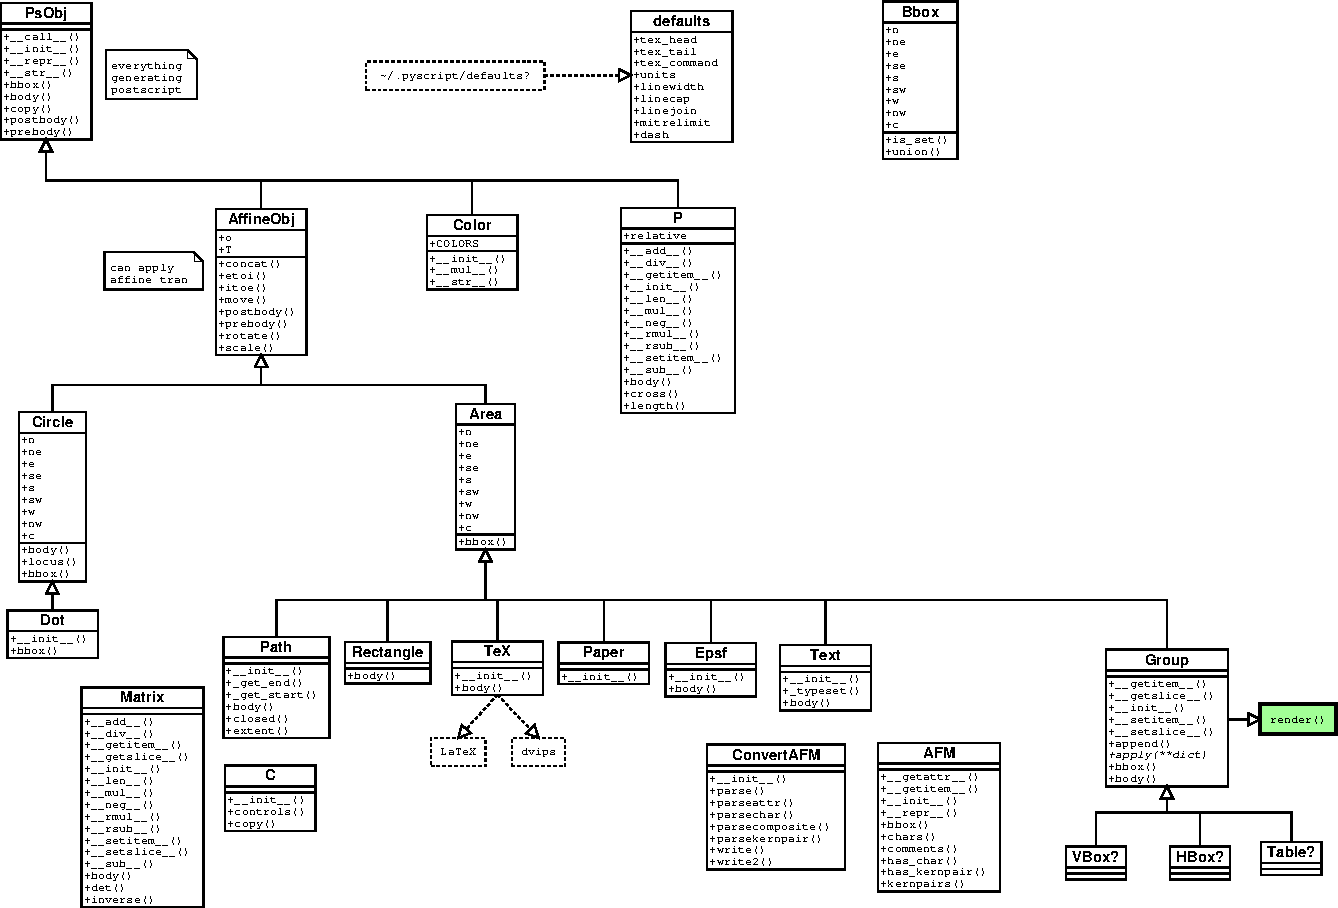
\includegraphics{class_structure}
  \end{center}
  \caption{Class structure of pyscript}
  \label{fig:classes}
\end{figure}

\section{Base Objects}

These are classes which add layers of functionality to pyscript objects.
Normally you wouldn't use these classes directly unless you're creating new 
pyscript objects. We'll decribe them here because they summarise what
you can do with pyscript objects.

%--------------------------------------------------------------------------
\subsection{PsObj()}
\label{sec:psobj}
\begin{python}
class PsObj(object):
    def __call__(self,**dict):
        Set a whole lot of attributes in one go

    def copy(self,**dict):
        return a copy of this object
        with listed attributes modified

    def __str__(self):
        return actual postscript string to generate object

    def body(self):
        subclasses should overide this for generating postscipt code

    def bbox(self):
        return objects bounding box
\end{python}

Base class which most (all?) \Verb|pyscript| classes are subclass.

A list of parameters can be set when an object is created with
calls like \Verb|t=Text('Hello',font='Helvetica')|
or by calling the object like a function as in \Verb|t(sw=P(0,2))|.
The parameters are also available singly as attributes: \Verb|t.sw| etc.

Printing an object produces the actual postscript code.

Objects may be copied with the \Verb|copy()| function and new
parameters can be passed in as arguments eg \Verb|s = t.copy(sw=P(0,0))|.

%--------------------------------------------------------------------------
\subsection{AffineObj()}
\label{sec:affineobj}
\begin{python}
class AffineObj(PsObj):

    o=P(0,0)
    T=Matrix(1,0,0,1)

    def concat(self,t,p=None):
        concat matrix t to tranformation matrix
          t: a 2x2 Matrix dectribing Affine transformation
          p: the origin for the transformation
          return: reference to self

    def move(self,*args):
        translate object by a certain amount
          param args: amount to move by, can be given as
            - dx,dy
            - P
          return: reference to self

    def rotate(self,angle,p=None):
        rotate object, 
        the rotation is around p when supplied otherwise
        it's the objects origin
          angle: angle in degrees, clockwise
          p: point to rotate around (external co-ords)
          return: reference to self

    def scale(self,sx,sy,p=None):
        scale object size (towards objects origin or p)
          sx sy: scale factors for each axis
          p: point around which to scale
          return: reference to self

    def itoe(self,p_i):
        convert internal to external co-ords
          p_i: intrnal co-ordinate
          return: external co-ordinate
        
    def etoi(self,p_e):
        convert external to internal co-ords
          p_e: external co-ordinate
          return: internal co-ordinate
\end{python}

A base class for objects that should implement affine transformations
(such as scaling, rotating etc), this should apply to any object that
draws on the page.


%--------------------------------------------------------------------------
\subsection{Area()}
\label{sec:area}
\begin{python}
class Area(AffineObj):

    o=P(0,0)
    width=0
    height=0

    n, ne, e, se, s, sw, w, nw, c  ... see description below
\end{python}

A Rectangular area defined by the south-west corner and the width and height.
This object mainly adds the ability to align to named compass points on the 
circumference see figure below.

\begin{center}
  \includegraphics{fig_area}
\end{center}

These points are always returned in external co-ordinates.

%--------------------------------------------------------------------------
\section{Drawing Objects}

%--------------------------------------------------------------------------
\subsection{Color()}
\label{sec:color}
\begin{python}
class Color(PsObj)
    def __mul__(self,other)
\end{python}

This class represents a postscript color. There are four ways to specify
the color distinguished by the number and type of paprameters that
are passed when you create the object.

\begin{itemize}
\item \Verb|Color(C,M,Y,K)| - a postsctipt CMYKColor (Cyan, Magenta, Yellow, blacK) 
\item \Verb|Color(R,G,B)| - RGBColor (Red, Green, Blue)
\item \Verb|Color(G)| - Gray
\item \Verb|Color('yellow')| etc
\end{itemize}

All the numbers above range from 0 to 1. Some of the named colors that
are defined are red, green, blue, cyan, magenta, yellow, black, white.

Color objects can be multiplied by a numeric factor between 0 and 1.
The effect is mostly to darken colors as they approach 0,
but this depends on how the colors where specified.
eg \Verb|Color(.2,.6,.6)*.5 = Color(.1,.3,.3)|

%--------------------------------------------------------------------------
\subsection{Rectangle()}
\label{sec:rectangle}
%\begin{python}
%\end{python}

\begin{center}
  \includegraphics{fig_rectangle}
\end{center}

%--------------------------------------------------------------------------
\subsection{Circle()}
\label{sec:circle}
%\begin{python}
%\end{python}

\begin{center}
  \includegraphics{fig_circle}
\end{center}

To obtain an ellipse, then just scale a circle.

\begin{example}
\begin{python}
d=Dot(P(0,0))
c1=Circle(n=d.c)
c2=Circle(fg=Color('green'))
c2[15]=d.c
render(d,c1,c2)
\end{python}
\begin{center}
  \includegraphics{fig_circle_eg1}
\end{center}
\end{example}

%--------------------------------------------------------------------------
\subsection{Dot()}
\label{sec:dot}
\begin{python}
class Dot(Circle):
    r=.1
    bg=Color(0)
    fg=None
\end{python}

A simple convenience function to draw a dot at the given location

%--------------------------------------------------------------------------
\subsection{Path()}
\label{sec:path}
%\begin{python}
%\end{python}

an abritrary path (line curve etc).

%--------------------------------------------------------------------------
\section{Text Objects}

%--------------------------------------------------------------------------
\subsection{Text()}
\label{sec:text}
%\begin{python}
%\end{python}
The \Verb|Text| object allows typesetting a simple string in a single
font.  The text will use \emph{kerning} automatically, that is, the
letter spacing will be adjusted depending on the pair of letters so
that it looks nicer. The kerning can be turned of if necessary, see
example below.
\begin{example}
\begin{python}
t1=Text('SWEPT AWAY',kerning=0,size=20)
t2=Text('SWEPT AWAY',kerning=1,size=20,nw=t1.sw)
render(t1,t2)
\end{python}
\begin{center}
  \includegraphics{text_kerning}
\end{center}
\end{example}

%--------------------------------------------------------------------------
\subsection{TeX()}
\label{sec:tex}
%\begin{python}
%\end{python}

%--------------------------------------------------------------------------
\section{Groups}

%--------------------------------------------------------------------------
\section{Vectors and Matrices}

%==========================================================================
\chapter{Development}

The aim of this section is to document some of the internals of
\Verb|pyscript| to enable developers to modify and extend it. 
It should also help in solving some of the trickier problems.


%--------------------------------------------------------------------------
\section{Object Attributes}
\label{sec:attributes}


\subsection{Native vs Dynamic}
\label{sec:native-vs-dynamic}

Initialisation and setting of the attributes is somewhat complicated.  We
want to be able to set attributes ala
\Verb|Text('font'='Helvetica',sw=P(0,-1))|, but to give full functionality
some attributes may need to be set on the fly, depending and affecting
others.  This is done with two types of attributes, \emph{native} which are
just dict entries and don't depend on anything else; and \emph{dynamic}
which are actually functions which return or set the native attibutes.

All classes that inherit from \Verb|PsDict| are dictionaries. 
The following functions are special and implement the dynamic attributes:
\begin{itemize}
\item \Verb|_get_name(self)|: the returned value of this fuction is what is
  returned from the call \Verb|obj['name']|
\item \Verb|_set_name(self,value)|: This function is executed by
  \Verb|obj['name']='bob'|

\end{itemize}
So to provide some dynamical attribute it is only neccessary to define 
the appropriately named functions. All classes in \Verb|pyscript|
should use this mechanism to provide a consistent feel to the user.

\subsection{Initialisation}
\label{sec:initialisation}

The class initialisation mechanism is motivated by the following
requirements:

\begin{itemize}
\item Each class should set all it's defaults for it's native attributes
\item Dynamic attributes can only be calculated/set after \emph{all} native
  attributes have been set, including base classes!.
\item Supplied attributes overide the defaults ... duh.
\end{itemize}

To initialise the attributes correctly classes should first call
\Verb|native(defaults,param)| to initialise all default native values, then
call the initialisation of the parent class eg:
\begin{python}
def __init__(self,**dict):
   
   ...code to calculate native attributes...

   self.natives({"width":0,"height":0},dict)
   apply(PsObject.__init__,(self,),dict)

   ...further initialisation...
\end{python}



%--------------------------------------------------------------------------
\section{Co-ordinates and Affine Transformations}
\label{sec:co-ordinates-affine}

Abritrary affine transformations (eg rotations, scaling, shearing,
reflection) can be applied to any object that is a subclass of 
\Verb|PsObject|. The way it is implemented in postscript is that the 
transformation is applied to the co-ordinate system \emph{before}
the object is drawn. Hence the placement of the object on the page
is actually a displacement of the \emph{internal} origin.

There are two co-ordinate systems for each object. An \emph{internal}
co-ordinate system in which the object is drawn. Usualy the origin (0,0) is
somewhere convenient on the object. There is also an \emph{external}
co-ordinate system which takes into account the placement, scaling etc of
the object. Co-ordinates can be converted from \emph{internal} to
\emph{external} using the member function \Verb|itoe(point)| and vice-versa
with \Verb|etoi(point)|.

Points that are returned from an object (eg \Verb|area.nw|) should
always be in the \emph{external} co-ordinates. Inparticular the origin,
\Verb|obj.o| is always in \emph{external} co-ordinates [internally it
just the point (0,0)]

%--------------------------------------------------------------------------
\section{Bounding Box}
\label{sec:bounding-box}

All objects subclassing \Verb|PsObject| must provide a \Verb|boundingbox()|
function which returns the SW and NE points of a tight bounding box for the
object (in \emph{external} co-ordinates). The bounding box will be used
to calculate the boundingbox for the entire drawing as way as allowing
the precise placement of objects.


%--------------------------------------------------------------------------
\section{Postscript Objects}
\label{sec:postscript-objects}

The basic class for implementing an object drawn directly in postscript
is \Verb|PsObject|. 

\appendix

\include{pyscriptQuantInfo}

% $Id$

\chapter{PyScript Plotting Package}



\end{document}
